\documentclass[12pt,a4paper,titlepage,portrait,openany]{book}
\usepackage[left=4cm, right=4cm, top=2cm, bottom=2cm]{geometry}
\usepackage[utf8]{inputenc}
\usepackage[english]{babel}
\usepackage{amsmath}
\usepackage{amsfonts}
\usepackage{amssymb}
\usepackage{graphicx}

\author{\text{A lesson note by}~Sewade O. Ogun}
\title{
\includegraphics[width=0.5\linewidth]{logo} \\\textbf{Foundations of Machine Learning}
}
\date{\today, \text{AIMS Ghana}}

\begin{document}
	\maketitle
	\tableofcontents
	\begin{table}[]	
		\begin{tabular}{ll}
			\title \textbf{{Symbols and Notations}} \\\\
			$\theta_i$  & Parameter i \\
			$\Theta$ & Set of Parameters         \\
			$n$ & Number of examples        \\
			$d$ & Number of features         \\
			$x_i$ & Single example at row i \\
			$x_i^j$ & Value of feature j at row i \\
			$y$ & Array of targets \\
			$X$ & Matrix of examples \\
			$D$ & Dataset consisting of $X,y$ \\
			$\mathcal{L}$ & Likelihood \\
			$\ell$ & Log-Likelihood \\
			$L$ & Loss of the function \\
			$\partial$ & Partial derivative \\
			$\nabla$ & Gradient \\
			$\lambda$ & preconditioner \\
			$\alpha$ & Learning rate \\
			$\mathbf{U}$ & Universal Set \\
			$\mathcal{O}(n)$ & Worse case complexity, BigO
			
		\end{tabular}	
	\end{table}

	\chapter{Supervised Learning}
	\section{Regression Problem}
	
	Given a set of datapoints, $ D = \left\{\left(X_i, y_i\right)\right\}_{i=1}^n $ where $x_i$ are the features and $y_i$ are the target, corresponding to the features, we can learn a function or hypothesis which maps the features $x_i$ to the target $y_i$ i.e $h : \mathbb{R}^d \to \mathbb{R}^c $
	\begin{table}[]\label{data_table}
		\begin{tabular}{|l|l|l|l|}
			\hline
			\textbf{} & \textbf{Weight (kg)} & \textbf{Color} & \textbf{Price (NGN)} \\ \hline
			x1                & 2.5                  & 0.8            & 1000                 \\ \hline
			x2                & 1.3                  & 0.2            & 800                  \\ \hline
			x3                & 3.7                  & 0.6            & 1700                 \\ \hline
			x4                & 1.4                  & 700            & ...                  \\ \hline
		\end{tabular}
	\caption {Table showing features and target of measurements gotten from observing tubers of yam sales. }
	\end{table}
	From table \ref{data_table}, Weight and Color are the features we wish to use to predict Price given the observations. This called a supervised learning task as the target is known.\\
	Given the supervised learning task, it is necessary to understand the given problem at hand by evaluating the following; \\
	\begin{enumerate}
		\item [a.] Data
		\item [b.] Hypothesis or model or Hypothesis class e.g. Regression
		\item [c.] Criteria (Loss, Cost)
		\item[d.] Learning Algorithm
	\end{enumerate}
\begin{center}
	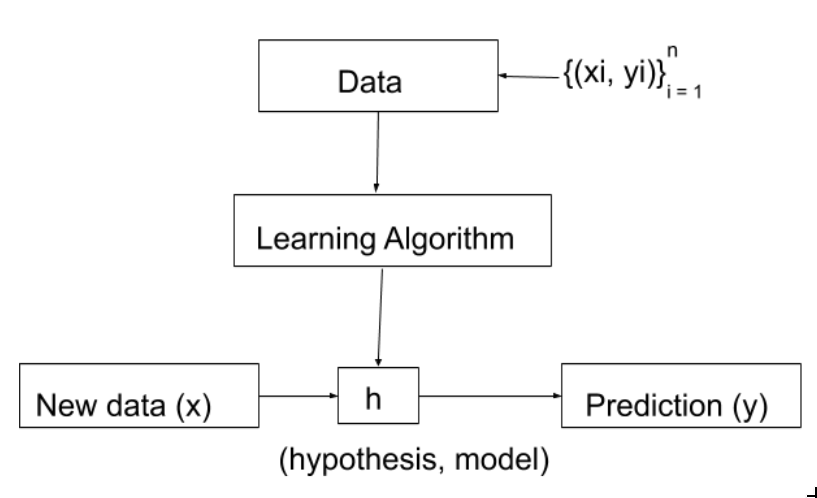
\includegraphics[width=0.6\linewidth, height=0.18\textheight]{model}
\end{center}
	
	\subsection{Hypothesis}
	The hypothesis function is \\
	\begin{equation}
		h_{\theta}(X) = \theta_0 + \theta_1x_1 + \theta_2x_2 + ... + \theta_nx_n
		= \sum_{i=0}^{n}\theta_ix_i \qquad (x_0=1)
	\end{equation}
	where $\theta$s are parameters of the model and $\theta_0$ is referred to as the \textbf{bias/intercept term}. Since this model has parameters, and the goal is to find the best parameters for the data, this form of models are referred to as \textbf{parametric models}. The other form are called \textbf{non-parametric models}.
	
	\subsection{Criteria}
	The criteria for the linear regression model is called \textbf{Ordinary Least Squares (OLS) or Mean Squared Error} because of the form of the criteria.  This is given as;
	\begin{equation}\label{loss_function}
	L(\theta) = \dfrac{1}{2}\sum_{i=1}^{n}\left(h_\theta(x_i) - y_i\right)^2
	\end{equation}
	
	\subsection{Learning Algorithm}
	The goal of the learning algorithm is to find the parameters $\theta$ that minimizes the loss function i.e. \\ $$ \min\limits_{\theta}L(\theta) = \dfrac{1}{2}\sum_{i=1}^{n}\left(h_\theta(x_i) - y_i\right)^2 $$
	Two approaches (Analytical method or Numerical methods) can be used to solve this problem.
	
	\subsubsection{Numerical Approach}
	Let $\Theta$ be the vector of $\theta$s and $Theta_0$ the initial solution, we can update $\Theta$ by repeatedly subtracting the gradient of the loss function from $\Theta$ until convergence i.e. \\
	Repeat 
	\begin{equation}\label{gradient descent}
	\theta_j := \theta_{j-1} - \alpha\dfrac{\partial}{\partial\theta_{j-1}}L(\theta_{j-1})
	\end{equation} where $\alpha$ is the \textbf{learning rate} and is an hyperparameter to be tuned.
	This form of learning in \eqref{gradient descent} is known as \textbf{gradient descent}. It involves taking steps in the opposite direction of steepest ascent gotten through the gradient.
	
	\subsubsection{Computing the Gradient of Loss Function}
	For one example, $h_\theta(x_i) = \Theta{x_i}$
	\begin{equation*}
	\begin{array}{cl}
	\dfrac{\partial}{\partial\theta}L(\theta) &= \dfrac{\partial}{\partial\theta} \dfrac{1}{2}\left(h_\theta(x_i) - y_i\right)^2 \\
	\\
	&= \dfrac{\partial}{\partial\theta} \dfrac{1}{2}\left(\theta_i{x_i} - y_i\right)\dfrac{\partial}{\partial\theta}\left(\theta{x_i - y}\right) \\\\
	&= \left(\theta_i{x_i} - y_i\right)x_i^j \\\\
	&= \left(h_\theta(x_i) - y_i\right)x_i^j
	\end{array}
	\end{equation*} where $x_i^j$ is the jth feature of the ith example. Therefore the update rule can be modified as;
	$\theta_j = \theta_{j} + \alpha(y_i - h_\theta(x^{(i)}))x_i^j$.
	The equation indicates that for a fixed learning rate, the amount of update is dependent on the difference between predictions and target. This is called the \textbf{Widrow-Hoff update rule} or \textbf{least mean square rule}.
	
	\subsubsection{Batch Gradient Descent}
	Gradient descent in general assumes that the loss function is differentiable and convex. If the loss function is not convex, the solution might get stuck in a local optimum and not find the global optimum. For linear regression, we can show that the loss function is convex as it is a function of 2nd polynomial and positive. \\ 
	The batch gradient descent uses all the examples on each iteration to compute the gradient. For a large set of examples, this can be computationally expensive and not used in practice. This also requires that the gradient is computed for every example before making one step of gradient descent. 
	\\
	${}\hspace{30pt} \text{Repeat until convergence;} $\\
	${}\hspace{50pt} \Theta = \Theta + \alpha\sum_{i=1}^{n}\left(y_i - h_\theta(x^{(i)})\right)x_i^j $
	
	\subsubsection{Stochastic Gradient Descent}
	Stochastic gradient descent selects a sample at random from the examples and uses this to update the gradient. This has the advantage of being fast and requiring less memory but does not guarantee convergence to the optimal solution (even though an approximate solution is usually good enough in practise) after the update. Also, update is not smooth as the direction of descent is dependent on only one data which may be noisy. \\
	${}\hspace{30pt} \text{Repeat until convergence;} $\\
	${}\hspace{50pt} \text{for i in 1 to n;} $
	
	${}\hspace{60pt} \Theta = \Theta + \alpha\left(y_i - h_\theta(x^{(i)})\right)x_i^j $
	
	\subsubsection{Mini-batch Stochastic Gradient Descent}
	A compromise between batch gradient descent and stochastic gradient descent is the mini-batch gradient descent. It uses a mini-batch of examples samples at random from the dataset  to update the parameters. This has the advantage of reducing the variance during update and therefor smoother. It also maximixes the usage of hardware and cpu vectorization for efficient computations. \\ \\
	${}\hspace{30pt} \text{Repeat until convergence;} $\\
	${}\hspace{50pt} \text{for k in 1 to no. of minibatches;} $
	 
	${}\hspace{60pt}\Theta = \Theta + \alpha\sum_{i=1}^{mbs}\left(y_i - h_\theta(x^{(i)})\right)x_i^j $\\
	where $mbs$ is the minibatch size.
	 	
	\subsubsection{Analytical Method}
	The analytical method performs a single computation using the data matrix. It the does not require to be performed iteratively and does not require a learning rate.
	\begin{equation*}
		\begin{array}{cl}
		L(\theta) &= \dfrac{1}{2}\|X\Theta - y\|^2 \\\\
		&= \dfrac{1}{2}(X\Theta - y)^T(X\Theta - y) \\\\
		&= \dfrac{1}{2}(\Theta^{T}X^T - y^T)(X\Theta - y) \\\\
		&= \dfrac{1}{2}(\Theta^{T}X^T - y^T)(X\Theta - y) ~ \text{as} ~ (A - B)^T = A^T - B^T \text{and} ~ (AB)^T = B^TA^T \\\\
		&= \dfrac{1}{2}(\Theta^{T}X^TX\Theta - 2y^TX\Theta + y^Ty)
		\end{array}
	\end{equation*}
	The gradient of $L(\Theta)$ is then computed as;
	\begin{equation*}
		\nabla_\theta = \dfrac{1}{2}\left(2X^TX\Theta - 2X^Ty\right)
	\end{equation*}
	\begin{equation*}
	X^TX\Theta = X^Ty
	\end{equation*}
	\begin{equation}\label{normal_eqn}
	\Theta = \left(X^TX\right)^{-1}X^Ty
	\end{equation}
	\eqref{normal_eqn} is known as the \textbf{normal equation} and requires the inverse of $X^TX$ to be computed. $X^TX$ may not be invertible and can be expensive to compute depending on the size of the dataset. To avoid the invertibility problem, the pseudoinverse can be computed and we can manually remove correlated features (by computing correlation matrix) if the features are linearly dependent. Another approach is to add regularization. To regularize the model, the sum of squares of the parameters is added to the loss function. This has the effect of also reducing the size of values of the parameters if the \textbf{regularization parameter} $\lambda$ is set appropraitely.
	
	
	\begin{equation}
	L(\theta) = \dfrac{1}{2}\|X\Theta - y\|^2 + \lambda\left\|\Theta\right\|_2^2
	\end{equation}
	\begin{equation}
		\Theta = \left(X^TX + \lambda{I}\right)^{-1}y^TX
	\end{equation}
	The proof of these regularization is shown in a later chapter using the Maximum a posteriori extimation(MAP). $I$ is the identity matrix and $\left(X^TX + \lambda{I}\right)^{-1}$ always exist
%	$\{(x^2+y^4)\}$ $\left\{\left(x^2+y^4\right)\right\}$
	
	\subsubsection{Newton's Method}
	The newton's method is a second-order optimization algorithm.
	Consider the diagram \ref{fig:loss-landscape} below,  
	
	\begin{figure}
		\centering
		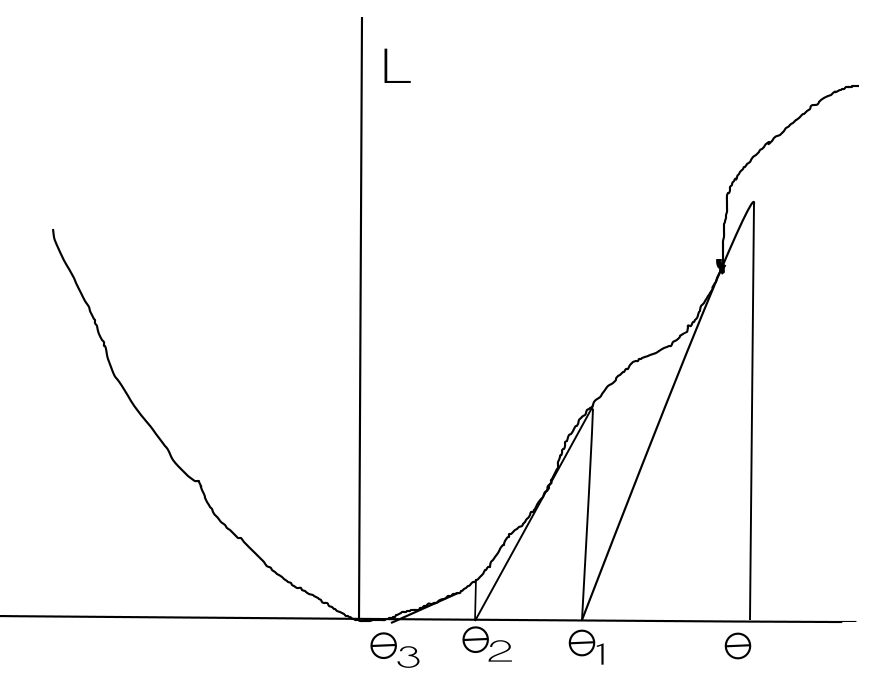
\includegraphics[width=0.7\linewidth, height=0.3\textheight]{loss-landscape}
		\caption{Newton Method showing theta update}
		\label{fig:loss-landscape}
	\end{figure}
	
	
	We want to find the point on the curve where the function is a minimum. Newton's method gives the formula as $\Theta := \Theta - \dfrac{f(\theta)}{f_i}$. For our machine learning task, this implies looking for the parameters $\Theta$ where the gradient is zero. 
	$$g = f^,$$ $$g^, = f^{,,}$$
	$$\Theta := \Theta - \dfrac{g}{g_i}$$
	$$\Theta := \Theta - \dfrac{f^,(\theta)}{f^,,(\theta)}$$
	In vecorized form, $\Theta := \Theta - H^{-1}\nabla_\theta\mathcal{L}$ where $H_{ij} = \dfrac{\partial}{\partial_{\theta_i}\theta_j}\mathcal{L}(\Theta)$. $H_{ij}$ is the second partial derivative $wrt$ all the $\Theta$s and is called \textbf{Hessian matrix}. If $x \in \mathbb{R}^{(n, d)}$, the $H \in \mathbb{R}^{(d, d)} $ \\
	
	\begin{enumerate}
		\item Newton's method is faster than stochastic gradient descent and converges in polynolial time.
		\item It requires no learning rate and instead takes into account the curvature of the loss function during optimization.
		\item A disadvantage is that inverting the Hessian is computationally expensive and the bigO is dependent on the number of parameters; $\mathcal{O}(d^2)$ 
		\item To make Hessian invertible where the matrix is singular, a preconditioner is applied; $H = H + \varepsilon{I}$ where $\varepsilon$ is a small number and values range from $10e^{-8}$ to $10e^{-10}$ in practise.
	
	\end{enumerate}
	\subsection{Maximum Likelihood Estimation}
	Maximum Likelihood estimation is a way of estimating the best parameters of a model given the data by maximizing the probability of the data.\\
	Given that $y_i = \Theta^Tx^i + \varepsilon_i$
	where $\varepsilon_i \sim \mathcal{N}(0, \sigma^2)$; the features are assumed to be centered with $\mu = 0$ and $\varepsilon_i$ is the difference between predictions and target which is a random variable and is Independently and Identically Distributed (IID). \\
	We know that for a normally distibuted random variable, $$PDF = \dfrac{1}{\sqrt[2]{2\pi\sigma^2}}e^{-\dfrac{(x_i-\mu)^2}{2\sigma^2}}$$ \\
	Since $\varepsilon_i$ is assumed to be normally distributed, 
	$$P(\varepsilon_i) = \dfrac{1}{\sqrt[2]{2\pi\sigma^2}}e^{-\dfrac{\varepsilon_i^2}{2\sigma^2}}$$
	$$P(\varepsilon_i) = \dfrac{1}{\sqrt[2]{2\pi\sigma^2}}e^{-\dfrac{(y_i - h_\theta(x_i))^2}{2\sigma^2}}$$
	For one example, $P(y_i | x_i;\Theta) = P(\varepsilon_i)$ and is read as Probability of $y_i$ given $x_i$ parameterized by theta equals probability of the error in estimation. For all examples,
	$$\prod_{i=1}^{n}P(y_i | x_i; \Theta) = \prod_{i=1}^{n}\dfrac{1}{\sigma\sqrt{2\pi}}e^{\dfrac{-(y_i - h_\theta(x_i))^2}{2\sigma^2}}$$
	
	Taking the log of both sides, (to eliminate the exponent),
	$$log \sum_{i=1}^{n}P(y_i | x_i;\Theta) = log \sum_{i=1}^{n}\dfrac{1}{\sigma\sqrt{2\pi}} + \sum_{i=1}^{n}-\dfrac{(y_i - h_\theta(x_i))^2}{2\sigma^2}$$
	Combining all the constant elements of the equation,
	$$P(y_i | x_i;\Theta) = \sum_{i=1}^{n}-\dfrac{(y_i - h_\theta(x_i))^2}{2\sigma^2} + C$$ since logarithm of a function is a monotonically increasing transformation of the function. 
	
	\textbf{Maximixing} the log likelihood of $P(y_i | x_i; \Theta)$ is equivalent to \textbf{minimizing} the loss.
	$$\min\limits_\theta{L(\Theta) }= \sum_{i=1}^{n}(y_i - h_\theta(x_i))^2$$ and is same output as the criteria specified in \eqref{loss_function}.
	
	\section{Classification Problem}
	Given a set of datapoints, $ D = \left\{\left(X_i, y_i\right)\right\}_{i=1}^n $ where $x_i$ are the features and $y_i$ $\in$ \{0, 1\} or $y_i$ $\in$ \{-1, 1\}  are the targets, corresponding to the features. In regression, the goal is to estimate a continuous variable while the estimated targets in classification are discrete. If $y$ has two classes, it is called \textbf{binary classification} while for classes greater than two, it is called \textbf{multi-class classification}.   The goal is to learn  a function or hypothesis which maps the features to classes $y$. \\
	 
	 
	\subsection{Hypothesis}
	\subsubsection{Logistic Regression}
	Logistic regression aims to fit a linear hyperplane separating the datapoints. An \textbf{hyperplane} is 1 dimension less than the plane in which it lives. 

	\begin{figure}
		\centering
		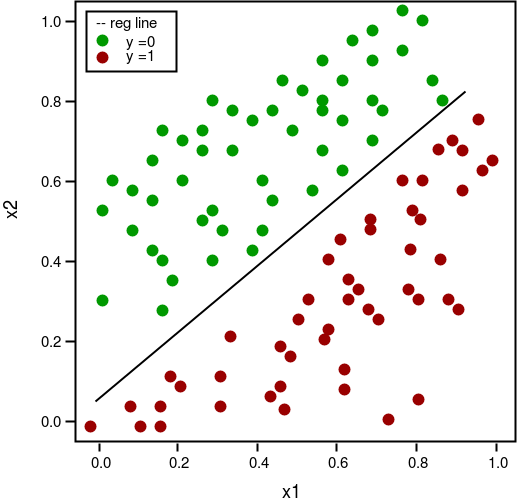
\includegraphics[width=0.8\linewidth ]{logistic-regression}
		
		\caption[]{Diagram Showing Hyperplane separating the two classes\protect\footnotemark}
		\label{fig:logistic-regression}
	\end{figure}
	\footnotetext{https://www.geeksforgeeks.org/understanding-logistic-regression/}
	The hypothesis is given by  $h_\theta(x) = \dfrac{1}{1+e^{-\Theta^Tx}}$. This assures that the predictions are bounded by 0 and 1. The form of the hypothesis is referred to as the sigmoid function or the logistic function. The sigmoid function is shown in \ref{fig:sigmoid} and the general form is $$g(z) = \dfrac{1}{1+e^{-z}} $$
	
	\begin{figure}
		\centering
		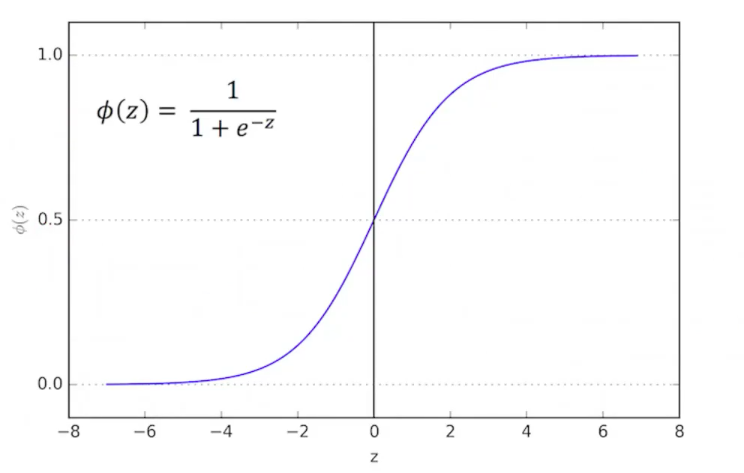
\includegraphics[width=0.7\linewidth]{sigmoid}
		\caption[Sigmoid]{Sigmoid Function\protect\footnotemark}
		\label{fig:sigmoid}
	\end{figure}
	\footnotetext{https://towardsdatascience.com/logistic-regression-a-simplified-approach-using-python-c4bc81a87c31}
	
	\subsection{Criteria}
	$$P(y = 1 | x;\Theta) = h_\theta(x)$$
	$$P(y = 1 | x;\Theta) = 1 - h_\theta(x)$$
	In compact form,
	$$P(y|x;\Theta) = h_\theta(x)^y * (1-h_\theta(\Theta))^{1-y}$$ 
	This equation relates to the bernoulli distribution equation. We can use the maximum likelihood estimation principle to get the criteria for the logistic regression as follows.
	$$\mathcal{L}(\Theta) = P(y|X;\Theta)$$
	$$\mathcal{L}(\Theta) = \prod_{i=1}^{n}P(y_i|x_i;\Theta)$$
	$$\mathcal{L}(\Theta) = \prod_{i=1}^{n}h_\theta(x_i)^{y_i} * (1-h_\theta(x_i))^{1-y_i}$$
	
	$$
		\mathcal{L}(\Theta) = \sum_{i=1}^{n}\left(y_ilog(h(x_i)) + (1-y_i)log(1-h_\theta(x_i))\right)
	$$
	In similar terms, maximizing the likelihood is equivalent to minimizing the negative log likelihood.
	$$arg\max\limits_{\theta}\mathcal{L}(\Theta) = arg\min\limits_{\theta}~-\mathcal{L}(\Theta)$$
	
	\begin{equation}\label{cross-entropy-loss}
	L(\Theta) = -\sum_{i=1}^{n}\left(y_ilog(h(x_i)) + (1-y_i)log(1-h_\theta(x_i))\right)
	\end{equation}
	
	\eqref{cross-entropy-loss} is known as the cross-entropy loss function. $\mathcal{L}(\Theta)$ is the log-likelihood and $L(\Theta)$ is the loss.
	
	\subsection{Learning Algorithm}
	Recall that $\Theta := \Theta + \alpha\nabla_\theta\mathcal{L}(\Theta)$ and $h_\theta(x) = g(\Theta^T\boldsymbol{x}) = \dfrac{1}{1+e^{-\Theta^T\boldsymbol{x}}}$
	
	$$
	\mathcal{L}(\Theta) = \sum_{i=1}^{n}\left(y_ilog(h(x_i)) + (1-y_i)log(1-h_\theta(x_i))\right)
	$$
	
	\subsubsection{Computing the Gradient}
	$$\dfrac{\partial}{\partial\theta}\mathcal{L}(\Theta) = \left(y\dfrac{1}{g(\Theta^Tx)} - (1-y)\dfrac{1}{1-g(\Theta^Tx)}\right).\dfrac{\partial}{\partial\theta_i}g(\Theta^Tx)$$
	
	$\text{But the derivative of sigmoid}~ g^1(z) = g(z).(1-g(z)) $ This implies
	
	$$\dfrac{\partial}{\partial\theta}\mathcal{L}(\Theta) = \left(y\dfrac{1}{g(\Theta^Tx)} - (1-y)\dfrac{1}{1-g(\Theta^Tx)}\right).g\left(\Theta^Tx\right)\left(1-g(\Theta^Tx)\right).\dfrac{\partial}{\partial\theta_i}\Theta^Tx$$
	
	$$\dfrac{\partial}{\partial\theta}\mathcal{L}(\Theta) = \left(y(1-g(\Theta^Tx)) - (1-y)g(\Theta^Tx)\right)x^j$$
	
	$$\dfrac{\partial}{\partial\theta}\mathcal{L}(\Theta) = (y-h_\theta(x))x^j$$
	The update rule for one example then becomes; \\\\
	${}\hspace{30pt} \text{Repeat until convergence;} $\\
	${}\hspace{50pt} \text{for i = 1 to n;} $\\
	${}\hspace{60pt} \Theta := \Theta + \sum_{i=1}^{n}\alpha (y_i - h_\theta(x_i))x_i^j$\\
	
	\subsubsection{Derivative of the sigmoid function}
	
	\begin{equation*}
	\begin{array}{cl}
		g(x) &= \dfrac{1}{1+e^{-x}} \\\\
		g^{'}(x) &= \dfrac{\delta}{\delta{x}} \left(1 + e^{-x}\right)^{-1} \\\\
		&= -1(1+e^{-x})^{-2}(-e^{-x}) \\\\
		&= \dfrac{e^{-x}}{\left(1+e^{-x}\right)^2} \\\\
		&= \dfrac{1}{\left(1+e^{-x}\right)}.\dfrac{(1+e^{-x})-1}{\left(1+e^{-x}\right)} \\\\
		&= \dfrac{1}{1+e^{-x}}.\left(\dfrac{1+e^{-x}}{1+e^{-x}} - \dfrac{1}{1+e^{-x}}\right) \\
		\\
		&= \dfrac{1}{1+e^{-x}}.\left(1 - \dfrac{1}{1+e^{-x}}\right) \\\\
		g^{'}(x) &= g(x).(1-g(x))
	\end{array}
	\end{equation*}
	
	\section{Risk Minimization}
	Given $(x_i, y_i)\sim P$ i.e. $x_i, y_i$ are samples observed from the probability distribution $P$, we want to minimize the expectation of squared errors. This is called the \textbf{True Risk Minimization}.
	$$\min\limits_{\theta}\mathbb{E}_{(x,y)\sim{P}} (h_\theta(x)-y)^2$$ \\
	Since we do not know the distribution and only have samples from it, we instead minimize the empirical equivalent known as the \textbf{Empirical Risk Minimization}.
	$$\min\limits_{\theta} \dfrac{1}{n} \sum_{i=1}^{n} (h_\theta(x)-y)^2$$ \\
	$y = h_{\theta^*}+\varepsilon$\\
	$h_{\theta^*}$ is the best prediction possible which we desire to find. \\
	$h_{\theta}$ is the prediction made by our model \\
	$\varepsilon \sim \mathbb{N}(0, \sigma^2)$ called the bayes\,(optimal) error\\
	
	\begin{equation}
	\begin{array}{cl}
		R_{h_\theta} &= \mathbb{E}[(y-h_\theta(x))^2] \\
		&= \mathbb{E}[(h_{\theta^*} + \varepsilon -h_{\theta}(x))^2] =
		\mathbb{E}[(\varepsilon + (h_{\theta^*}  -h_{\theta}(x))^2] \\
		\text{Let}~b = (h_{\theta^*}  -h_{\theta}(x))^2 \\
		&= \mathbb{E}[\varepsilon_i^2 + 2\varepsilon_i{b} + b^2] \\
		&= \mathbb{E}[\varepsilon^2] + \mathbb{E}[2\varepsilon_i{b}] + \mathbb{E}[b^2] \\
		\linebreak
		\text{Recall;} \\
		Var(x) &= \mathbb{E} - [\mathbb{E}(x)]^2 \\
		&= \mathbb{E}[(x - \mu)^2] ~ \text{where} ~ \mathbb{E}(x) = \mu \\
		&= \mathbb{E}(x^2 -2\mu{x}+\mu^2) \\
		&= \mathbb{E}(x^2)-2\mu\mathbb{E} + \mu^2 \\
		&= \mathbb{E}(x^2)-2\mu^2 + \mu^2 \\
		&= \mathbb{E}(x^2) + \mu^2 \\
		&= \mathbb{E}(x^2)-[\mathbb{E}(x)]^2 \\\\
		\text{Plugging in Var}(x);
		R_{h_\theta} &= Var(\varepsilon) + [\mathbb{E}(\varepsilon)]^2 + 2\mathbb{E}(\varepsilon)\mathbb{E}(b) + Var(b) + [\mathbb{E}(b)]^2~\text{but}~\mathbb{E} = 0 \\
		&= Var(\varepsilon) + Var(b) + [\mathbb{E}(b)]^2 \\
		&= \sigma^2 + Var(b) + [\mathbb{E}(b)]^2 \\
		&= \sigma^2 + Var(h_{\theta^*}(x) - h_\theta{x}) + [\mathbb{E}(h_{\theta^*}(x) - h_\theta(x))]^2
				
	\end{array}
	\end{equation}
	The risk is composed of noise $\sigma^2$, bias
	$[\mathbb{E}(h_{\theta^*}(x) - h_\theta(x))]^2$ and variance $Var[h_{\theta^*}(x) - h_\theta{x}]$ of the model. The noise $\sigma^2$ is derived from the data and not under the model's control, and is also the minimum loss value our model can have. It is also a requirement to have low values for both variance and bias. \\\\
	Reducing the variance when training the model increases the bias of the model and vice-versa. The solution is to find a model with the right complexity which reduces the variance and bias simultaneously. This phenomenon is called the \textbf{Bias-Variance Tradeoff}.
	
	\subsection{Bias and Variance}
	A model is said to be overfitting  if it has a high variance and is seen where the training set loss is low while the validation set loss is high. A model is said to be underfitting if training set loss is high and validation set loss is also high.
	
	\begin{figure}
		\centering
		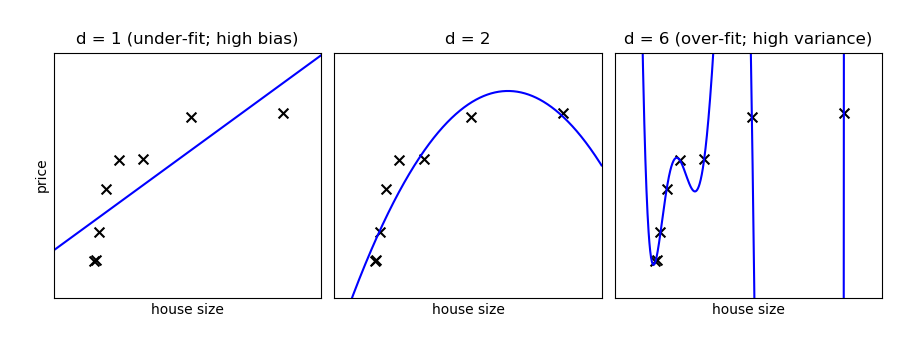
\includegraphics[width=\linewidth, height=0.26\textheight]{bias_variance}
		\caption[]{Diagram Showing Overfitting, Normal and Underfitting\protect\footnotemark}
		\label{fig:biasvariance}
	\end{figure}

	\footnotetext{https://scipy-lectures.org/packages/scikit-learn/auto\_examples/plot\_bias\_variance.html\#bias-and-variance-of-polynomial-fit}
	
	For high bias model, we can (1) train the model for a longer period (2) use a more complex model (3) increase the learning rate\\
	For high variance model, we can (1) get more training data (2) make the model simpler (3) reduce the number of features (4) add regularization. \\\\
	In practise, the data is split into training and validation sets (but slitting the data into two folds also has the effect of making us loose information in the validation set that could have been used by the model). \\
	
	To cater for the effect of data splitting, \textbf{cross-validation} method is used to choose the best model.
	
	\subsection{K-Fold Cross Validation}
	Given the set of data $D = \left\{(x_i, y_i)\right\}_{i=1}^m$ and the criteria such as $L(\theta) = \dfrac{1}{2}\sum_{i=1}^{n}\left(h_\theta(x_i) - y_i\right)^2$ for linear regression;
	\begin{enumerate}
		\item Randomly split $D$ into k disjoint subsets of size $\frac{m}{k}$
		$$D = \bigcup\limits_{i=1}^{k}D_i$$
		\item For each model $M_i$, \\
		${}\hspace{30pt} \text{For each j = 1, ..., k}$ \\
		${}\hspace{40pt}  \text{Train}~ M_{ij} on D - D_j$ \\
		${}\hspace{40pt}$  \text{Test on}~$D_j$ and compute $L_{D_j}(M_{ij})$
		\item Compute generalization error of $M_i$ = average of $L_{D_j}(M_{ij})$
		\item Pick the model $M$ with the lowest generalization error i.e. model that has reduced risk $R_{h_\theta}$
		\item Put all the data together i.e retrain $D$ using the best model.
	\end{enumerate}

	An extreme case of the K-Fold cross validation where all the data are split into n folds is called \textbf{Leave-One-Out Cross Validation}. In this case, only one example is used for validation at each instance and can be used when the number of examples, n is not large.
	
	\subsubsection{Hints}
	\begin{enumerate}
		\item Typically, $k = 10$ for large dataset and $k = 3$ for smaller dataset.
		\item Number of folds should be less than number of examples $k \leq n$
		\item If the number of examples is very large, say $n  = 1000000$, cross validation may not be necessary provided the validation set can be representative.
		
	\end{enumerate}
	
	\subsection{Reducing the Model Complexity}
	\subsubsection{Feature Selection}
	Feature selection is done to (1) reduce the model complexity (2) determine the features that are most predictive (3) reduce the number of features, preventing overfitting. \\
	For d features, the number of feature subsets = $2^d$.
	There are two feature selection methods, namely (1) Wrapper Methods (2) Filter Methods.
	\subsubsection{Feature Selection with Wrapper Methods}
	\begin{enumerate}
		\item[a.] \textbf{Forward Search}
		It begins with an empty set and proceeds to find most predictive combination of features from all the feature subsets.
		
		\textbf{Algorithm}
		\begin{enumerate}
			\item[1.] Intialize $F = \emptyset$
			\item[2.] Repeat \{
			\begin{enumerate}
				\item[a.] For i in range(d)
				\begin{enumerate}
					\item[-] if i $\notin F$, let $F_i=F\cup\{i\}$
					\item[-] Use cross-validation to evaluate $F_i$
				\end{enumerate}
				\item[b.] Set $F$ to be the best subset found at $(a)$
			\end{enumerate}
			\item[3.] Select the best subset that was found during the entire procedure.
		\} 
		\end{enumerate}
	For d features, complete forward search takes $\mathcal{O}(d^2)$\\
		\item[b.] Backward Search \\
		\textbf{Algorithm}
		\begin{enumerate}
			\item[1.] Initialize $F = \mathbf{U} $, the set of all features
			\item[2.] Repeat \{
			\begin{enumerate}
				\item[a.] For i in range(d)
				\begin{enumerate}
					\item[-] if i $\in F$, let $F_i=F - \{i\}$
					\item[-] Use cross-validation to evaluate $F_i$
				\end{enumerate}
				\item[b.] Set $F$ to be the best subset found at $(a)$
			\end{enumerate}
			\item[3.] Select the best subset that was found during the entire procedure.
			\}
		\end{enumerate}
	\end{enumerate}

	\subsubsection{Feature Selection with Filter Methods}
	Filter methods measure correlation between each feature and target. The features with more correlation are more predictive of the target variable. A type of correlation commonly used is called \textbf{Mutual Information}.
	$$MI(x^{(i)},y) = KL\left(P\left(x^{(i)}\right) || P\left(x^{(i)}P(y)\right)\right)$$
	where $MI$ is the mutual information, $KL$ is Kulback-Leibler Divergence (which is also known as relative entropy).
	
	$$\text{KL Distance,}~D_{KL}(X||y) = \sum_{i=1}^{n}\left[P(x_i)*log\dfrac{x_i}{y_i}\right]$$
	
	\textbf{Algorithm}
	\begin{enumerate}
		\item Compute MI
		\item Take k set of features with largest correlation
	\end{enumerate} 
	\textbf{Advantage: }Complexity of filter methods is linear with time i.e. $\mathcal{O}(d)$ for $d$ features. \\
	\textbf{Disadvantage: }It does not take into account cross-correlation between features. \\\\
	A combination of Wrapper method and filter method can be used to select the most predictive features, combining their relative strength.
	
	
	
	
	
	
	
	
	
\end{document}